\chapter{Force électrique}

\section{Charge électrique}

\marginpar{Tremblay \S 1.1 à 1.6}

\paragraph{Objectif}

\begin{enumerate}
  \item L'étudiant saura qu'il existe deux types de charges électriques et
    comprendra quelles expériences permettent de le démontrer.
  \item L'étudiant connaîtra le principes de conservation de la charge
    et saura l'appliquer pour résoudre des problèmes simples.
  \item L'étudiant connaîtra le principe de quantification de la charge et
    pourra l'appliquer pour résoudre des problèmes simples.
  \item L'étudiant comprendra la polarisation induite dans les isolants.
\end{enumerate}


\paragraph{Matériel}

\begin{enumerate}
  \item Tige de plastique
  \item Tige de verre
  \item Tige métallique
  \item Laine
  \item Fourrure
\end{enumerate}


\subsection*{Démonstration de l'existence de deux types de charges}

\marginpar{10 minutes}

\marginpar{Laine, fourrure, plastique, verre, support, métal}

\begin{enumerate}
\item Si on approche les deux tiges de plastique, rien ne se produit.
\item Si on frotte les deux tiges de plastique avec de la laine, elles se
  repoussent. Comme les deux tiges ont subi le même traitement, elles ont
  la même \textbf{charge}. Donc, \textbf{les charges identiques se
    repoussent}.
\item On répète avec les tiges de verre qu'on frotte avec la fourrure.
\item On frotte une tige de plastique et une tige de verre, elles
  s'attirent. Il semble donc que la charge de la tige de verre soit
  différente de celle de plastique et que \textbf{les charges opposées
    s'attirent}.
\item Si on approche la laine qui a chargé le plastique de la tige de
  verre,  elles se repoussent. Par conséquent la tige de plastique a
  transféré ses charges à la laine qui acquiert donc une charge identique à
  celle de la tige de verre.
\item Si on approche un objet métallique non chargé de la tige de plastique
  chargée, on constate une attraction. Le métal se charge par
  \textbf{induction} et l'extrémité proche de la tige de plastique acquiert
  une charge opposée à celle du plastique.
\end{enumerate}


\subsection*{Types de charge}
\marginpar{5 minutes}
\marginpar{Noter au tableau}

On appelle la charge du verre une charge \textbf{positive} et celle du
plastique une charge \textbf{négative}.

Deux objets avec le même type de charge se repoussent. Deux objets avec des
charges opposées s'attirent.

On notera souvent les charges électriques par des $q$ : $q$, $Q$, $q_1$, $q_2$,
\ldots.

L'unité SI pour la charge est le \textbf{coulomb} (C). La \textbf{charge
  élémentaire} est la charge du proton et vaut
$$e = \SI{1.602 176 634e-19}{\coulomb}.$$
\marginpar{Valeur exacte décidée le 16 novembre 2018, en application à partir
    du 20 mai 2019}
L'électron a une charge de $-e$.

Lorsqu'on charge par frottement, ce sont les électrons qui sont arrachés d'un
matériau et transféré à l'autre. Les protons sont \og cachés \fg au centre des
atomes.

Un objet \textbf{neutre} a autant de proton que d'électrons. La plupart des
objets dans l'univers sont neutres.


\subsection*{Question}

\marginpar{5 minutes}
\marginpar{Diapo}

Lorsqu'on frotte les tiges, des charges se déplacent entre
la tige et le tissu. La tige métallique n'a pas été frottée mais elle attire
néanmoins la tige de plastique chargée. Où sont les charges?

\marginpar{Noter au tableau}
On peut \textbf{induire} une redistribution de la charge dans un métal en
approchant un objet chargé. Aucune charge n'est transférée entre les deux
objets.

\subsection*{Principe de conservation de la charge}  %

\marginpar{10 minutes}
\marginpar{Noter au tableau}

La charge électrique totale dans un système fermé est toujours la même.

Par exemple, la charge est conservée lors de la désintégration d'un neutron
libre (temps de demi-vie d'environ \SI{10.3}{minutes}): $n \rightarrow p^+ +
e^- + \bar{\nu}_e$.



\subsection*{Quantification de la charge}
\marginpar{5 minutes}

La charge électrique ne peut prendre que des valeurs qui correspondent à des
multiples entier de la charge élémentaire ($e$, $10^{8}e$, $-45e$, etc.).


\subsection*{Question}
\marginpar{10 minutes}
\marginpar{Diapo}

Indiquez si chacune des réactions suivantes est possible.
  \begin{enumerate}
    \item \ce{H^+ + OH^- -> H_2O}
    \item $\pi^+ + p^+ \longrightarrow \Sigma^0 + K^+$
    \item \ce{^4_2He^{2+} + ^14_7N -> ^17_8O + p^+}
  \end{enumerate}


\subsection*{Question}
\marginpar{10 minutes}
\marginpar{Diapo}
Est-ce qu'un objet peut avoir les charges suivantes?

  \begin{enumerate}
    \item $q_1 = \SI{-2.05056e-17}{C}$
    \item $q_2 = \SI{3.74868e-18}{C}$
    \item $q_3 = \SI{4.00}{C}$
  \end{enumerate}


\sectionline


\section{Isolants et conducteurs}
\marginpar{10 minutes}
\marginpar{Tremblay \S 1.7 et 1.8}

  Dans le cas de l'objet métallique qui attire la tige de plastique chargée
  négativement, nous avons vu que des charges électriques se déplaçaient dans
  l'objet métallique.

  \vspace{0.3cm}
  Un \textbf{conducteur} est un matériau dans lequel les charges peuvent se
  déplacer rapidement. Un \textbf{isolant} est un matériau dans lequel les
  charges ont beaucoup de difficulté à se déplacer.

  \vspace{0.3cm}
  La différence entre les deux types par le \textbf{temps de relaxation},
  c'est-à-dire le temps que des charges mettent à se déplacer jusqu'à leur
  position d'équilibre.

  \vspace{0.3cm}
  Exemple: cuivre \SI{1e-12}{\second}, verre \SI{2}{\second}, polystyrène
  \SI{1e10}{\second}.



\subsection*{Objets conducteurs identiques en contact}
\marginpar{3 minutes}
  Si deux objets conducteurs identiques sont mis en contact, les charges
  qu'ils portaient seront très rapidement réparties également entre les deux
  objets.


\subsection*{Question}
\marginpar{5 minutes}
\marginpar{Diapo}
\marginpar{Électroscope}
Que se passe-t-il si on touche la partie du haut avec une tige chargée
négativement puis qu'on la retire?



\subsection*{Question}
\marginpar{10 minutes}
\marginpar{Diapo}
\marginpar{À ramasser}
Deux objets métalliques identiques ont des charges $Q$ et $-6Q$,
respectivement. Les deux objets sont mis en contact puis sont séparés. Quelles
sont les charges sur chacun des objets?

\vspace{0.3cm}
\marginpar{Solution détaillée}
La charge totale dans le système avant le contact est $Q + -6Q = -5Q$.

Par le principe de conservation de la charge, la charge totale après le contact
sera aussi de $-5Q$.

Puisque les deux objets sont des conducteurs, les charges (électrons) pourront
se déplacer d'un à l'autre.

Puisque les objets sont identiques la charge sur chacun d'eux après le contact
doit être la même.

Par conséquent, ils ont chacun la
moitié de la charge totale, soit $-\num{2.5}Q$.


\subsection*{Polarisation dans les isolants}
\marginpar{10 minutes}
\marginpar{Dessin, ballon}

Comment un ballon qu'on frotte sur ses cheveux peut-il tenir au mur si le
ballon et le mur sont des isolants?

Le ballons est chargé par frottement et acquiert une charge négative. Le mur
est neutre et isolant, donc les électrons ne sont pas libres de se déplacer.
Par contre, les atomes à proximité du ballon vont se réorganiser très
légèrement : le nuage d'électron s'éloignera du ballon alors que le noyau
s'en rapprochera. Les atomes seront \textbf{polarisés}. Puisque le ballon est
plus près des charges positives que des charges négatives, il y a une
attraction nette entre le ballon et le mur.

\begin{center}
\begin{tikzpicture}
\draw (3, 1.7) -- (3, -1.9);
\draw (2.298, -1.928) arc (-40:40:3);
\draw[decorate, decoration={markings,
                mark=between positions 0 and 1 step 8mm with {
                \node[circle, negative, minimum size=4mm] (0, 0) {$-$};}}]
    (1.915, -1.607) arc (-40:40:2.5);
\foreach \y in {1.7, 0.9, 0.1, -0.7, -1.5} {
  \draw[positive] (3.7, \y) arc (90:270:0.5 and 0.3) -- (3.7, \y);
  \node at (3.5, \y - 0.3) {$+$};
  \draw[negative] (3.71, \y - 0.6) arc (-90:90:0.5 and 0.3) -- (3.71, \y - 0.6);
  \node at (3.9, \y - 0.3) {$-$};
}
\coordinate (origin) (0, 0);
\draw[ultra thick, ->] (origin) -- (-1, 0) node[left] {$\vec{N}$};
\draw[ultra thick, ->] (origin) -- (1, 0) node[right] {$\vec{F}_e$};
\draw[ultra thick, ->] (origin) -- (0, 1.4) node[right] {$\vec{f}$};
\draw[ultra thick, ->] (origin) -- (0, -1.4) node[right] {$\vec{F}_g$};
\draw[draw=white,fill=white] (-0.02, -0.02) rectangle (0.02, 0.02);
\node at (-1, 1.7) {Ballon};
\node at(6, 1.7) {Mur};
\end{tikzpicture}
\end{center}

\subsection*{Exercice}
\marginpar{5 minutes}
Le coefficient de frottement entre le mur et le ballon est $0.6$, et la masse
du ballon est de \SI{2.9}{g}. Quel est
le module de la force électrique entre le ballon et le mur?


\sectionline


\subsection*{Solution de l'exercice}
\marginpar{15 minutes}

  $N = F_e$ car composante horizontale de l'accélération est nulle (équilibre).

  $f = \mu_s N = \mu_s F_e$.

  $f = F_g$ car composante verticale de l'accélération est nulle (équilibre).

  $\mu_s F_e = mg$

  $F_e = \frac{mg}{\mu_s} = 0.0474 N$


\subsection*{Charge par induction}
\marginpar{5 minutes}
\marginpar{Diapo}
  Nous avons parlé de charge par frottement. Il est également possible de
  charger un conducteur par induction.
  \begin{center}
    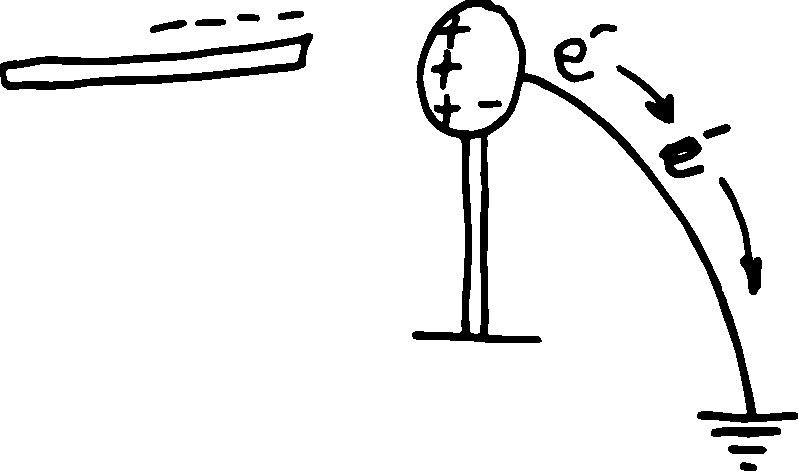
\includegraphics[height=3cm]{figures/charge-induction-3.pdf}
  \end{center}


%\paragraph{Matériel}

%\begin{enumerate}
  %\item Ballon
  %\item Balance à torsion pour loi de Coulomb
%\end{enumerate}


%\subsection*{Démonstration de la loi de Coulomb}
%\marginpar{15 minutes}
%\marginpar{Montage installé au labo}

  %Une boule métallique installée sur une balance à torsion.

  %Faire les manips suivantes dans l'ordre.

  %\begin{itemize}
    %\item Boules non chargées, mesurer position du laser et distance entre les
      %boules
    %\item Une boule chargée, mêmes mesures. La boule suspendue devrait se
      %rapprocher de la boule fixe puisqu'elle se polarise par induction.
    %\item Deux boules chargées. La boule suspendue devrait s'éloigner de la
      %boule fixe car des charges de même signe se repoussent. Disons que la
      %distance entre les boules est $r$ et la position du laser s'est déplacée
      %de $d$.
    %\item Si on déplace la boule fixe à $2r$, la force de répulsion entre les
      %deux boules diminue d'un facteur $4$ et le laser devrait être à une
      %distance $d/4$ de sa position d'équilibre.
    %\item On remet la boule fixe à sa position initiale,$r$. On touche la boule
      %fixe avec une troisième boule identique qu'on retire. La charge de la boule fixe passe
      %donc de $Q$ à $Q/2$. La force entre les deux boules diminue donc de
      %moitié et on devrait voir le pointeur laser se déplacer à $d/2$.
  %\end{itemize}

\newpage

\section{Loi de Coulomb}

\marginpar{Tremblay \S 1.9}

\paragraph{Objectif}

\begin{enumerate}
  \item L'étudiant comprendra la loi de Coulomb et comment cette loi capture
    toutes les observations faites précédemment au sujet des charges.
  \item L'étudiant pourra faire des calculs de forces électrostatiques.
  \item L'étudiant comprendra le principe de superposition.
\end{enumerate}


\subsection*{Observations clés}
\marginpar{10 minutes}
  \begin{itemize}
    \item charges opposées s'attirent
    \item charges de même signe se repoussent
    \item plus la charge est grande, plus la force est grande
    \item plus les charges sont éloignées, plus la force est petite
  \end{itemize}

  La loi de Coulomb capture tous ces éléments.

  Considérons deux charges $q_1$ et $q_2$ séparées d'une distance $r$.

    \begin{center}
    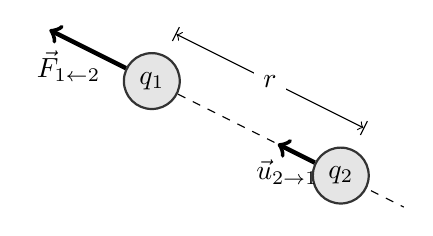
\begin{tikzpicture}[
      charge/.style={circle, draw=black!80, fill=black!10, thick}]
      \draw[dashed] (0, 2) -- (4, 0);
      \node[charge] (q1) at (0.8, 1.6) {$q_1$};
      \node[charge] (q2) at (3.2, 0.4) {$q_2$};
      \draw[|<->|] (1.1, 2.2) -- node[fill=white] {$r$} (3.5, 1);
      \draw[ultra thick, ->] (q1) -- node[near end, below] {$\vec{F}_{1
          \leftarrow 2}$} (-0.5, 2.25);
      \draw[ultra thick, ->] (q2) -- node[near end, below]
      {$\vec{u}_{2 \rightarrow 1}$} (2.4, 0.8);
    \end{tikzpicture}
    \end{center}
  On doit avoir
  \begin{eqnarray*}
    F_{1 \leftarrow 2} & \propto & \abs{q_1}, \\
    F_{1 \leftarrow 2} & \propto & \abs{q_2}, \\
    F_{1 \leftarrow 2} & \propto & \frac{1}{r^\gamma}.
  \end{eqnarray*}
  Autrement dit,
  $$
    F_{1 \leftarrow 2} = \frac{k\abs{q_1 q_2}}{r^\gamma}.
  $$
  où $k$ est une constante de proportionnalité. L'exposant peut être trouvé
  expérimentalement. C'est ce qu'à fait Charles Augustin de Coulomb. L'exposant
  est $2$, soit le même que celui qui apparaît dans la loi de la gravitation
  newtonienne.

  Pour spécifier l'orientation, nous utilisons un vecteur unitaire $\vec{u}_{2
  \rightarrow 1}$ qui pointe de la charge $q_2$ vers la charge $q_1$. Si les
  deux charges sont de même signe, la force est répulsive et la force sur $q_1$
  est dans la même direction que $\vec{u}_{2 \rightarrow 1}$. On note que
  $q_1q_2$ est positif. Donc
  $$\vF_{1 \leftarrow 2} = \frac{kq_1q_2}{r^2}\vec{u}_{2 \rightarrow 1}$$

  Trouver les unités par analyse dimensionnelle.
  $$k = \frac{1}{4\pi\epsilon_0} = \SI{8.99e9}{N m^2 / C^2}$$
  $$\epsilon_0 = \SI{8.854e-12}{C^2 / N m^2}$$



\subsection*{Exercice}
\marginpar{20 minutes}
  Deux charges immobiles $q_1 = \SI{4.00}{nC}$ et $q_2 = \SI{-6.00}{nC}$ sont
  situées à \SI{5}{cm} l'une de l'autre.
  Est-il possible de placer une troisième charge le long de la droite reliant
  $q_1$ et $q_2$ de telle sorte qu'elle soit à l'équilibre?


\sectionline


\paragraph{Solution}

D'abord, on fait un schéma de la situation. Imaginons que la charge qu'on
ajoute est positive. La direction de la force exercée par $q_1$ et $q_2$ dans
différentes régions est indiquée sur la figure.

\begin{center}
\begin{tikzpicture}[
      charge/.style={circle, draw=black!80, fill=black!10, thick}]
  \draw[->] (-2, 0) -- (4, 0) node[below] {$x$};
  \node[circle, positive] (q1) at (0, 0.5) {$q_1$};
  \node[circle, negative] (q2) at (3, 0.5) {$q_2$};
  \node[charge] (q) at (-1.5, 0.5) {$q$};
  \draw (q1|-0,0) -- ++(0, -0.2) node[below] {$0$};
  \draw (q2|-0,0) -- ++(0, -0.2) node[below] {$d$};
  \draw (q|-0,0) -- ++(0, -0.2) node[below] {$x$};
  % Forces by q1
  \draw[ultra thick, ->, positive] (-0.3, 1.2) -- ++(-1, 0);
  \draw[ultra thick, ->, positive] (1, 1.2) -- ++(1, 0);
  \draw[ultra thick, ->, positive] (3.3, 1.2) -- ++(1, 0);
  % Forces by q2
  \draw[ultra thick, ->, negative] (-1.3, 1.5) -- ++(1, 0);
  \draw[ultra thick, ->, negative] (1, 1.5) -- ++(1, 0);
  \draw[ultra thick, ->, negative] (4.3, 1.5) -- ++(-1, 0);
\end{tikzpicture}
\end{center}

À gauche de $q_1$, les deux forces sont opposées et la plus grande charge en
valeur absolue est plus éloignée. Il est possible que les deux forces
s'annulent.

Entre $q_1$ et $q_2$, les deux forces sont dans la même direction : elles ne
peuvent pas s'annuler.

À droite de $q_2$, les deux forces sont opposées et la plus grande charge en
valeur absolue est plus proche. Il est impossible que les deux forces
s'annulent.

On conclut donc que la position recherchée est pour une valeur $x$ négative. La
distance entre la nouvelle charge $q$ et $q_1$ est donc $\abs{x}$ alors que la
distance entre $q$ et $q_2$ est de $d - x$. On peut calculer le module de la
force exercée par $q_1$ et $q_2$ sur $q$ ainsi que les composantes.
\begin{align*}
  F_1 &= \frac{k\abs{q_1q}}{x^2}        &  F_{1x} &= -\frac{kq_1q}{x^2} \\
  F_2 &= \frac{k\abs{q_2q}}{(d - x)^2}  &  F_{2x} &= -\frac{kq_2q}{(d - x)^2}
\end{align*}

La force nette sur $q$ est nulle car on veut que cette particule soit à
l'équilibre.  Par le principe de superposition, la force nette sur $q$ est
\begin{align*}
     F_x &= F_{1x} + F_{2x} \\
         &= 0  \\
  F_{1x} &= -F_{2x} \\
  -\frac{kq_1q}{x^2} &= \frac{kq_2q}{(d - x)^2} \\
  -\frac{q_1}{x^2} &= \frac{q_2}{(d - x)^2} \\
  x^2q_2 + q_1(d - x)^2 &= 0 \\
  x^2q_2 + q_1d^2 - 2q_1dx + q_1x^2 &= 0 \\
  (q_1 + q_2) x^2 - 2 q_1 d x + q_1d^2 &= 0 \\
  x &= \frac{2q_1 d \pm \sqrt{4q_1^2d^2 - 4(q_1 + q_2) q_1 d^2}}{2(q_1 + q_2)}
\end{align*}
Les deux réponses possibles sont $x = \SI{-22.25}{cm}$ et $x = \SI{2.247}{cm}$.
On sait que la particule doit être à gauche de $q_1$, donc la bonne solution
est $x = \SI{-22.25}{cm}$.



\subsection*{Exercice}
\marginpar{15 minutes}

  \textit{Laisser les étudiants travailler sur ce problème avant de faire la
    solution avec eux.}

  \textit{Cet exemple rappelle le principe de superposition.}

  On considère l'ensemble de charges représenté ci-dessous. Les charges sont
  immobiles.

  \begin{center}
  \begin{tikzpicture}[scale=1]
    \node[circle, positive] at (0, 2) (q1) {$q_1$};
    \node[circle, positive] at (0, 0) (q2) {$q_2$};
    \node[circle, positive] at (5, 0) (q3) {$q_3$};
    \node[circle, positive] at (5, 2) (q4) {$q_4$};
    \draw[<->] (q1) -- node[fill=white] {$l$} (q2);
    \draw[<->] (q2) -- node[fill=white] {$d$} (q3);
  \end{tikzpicture}
  \end{center}

  \begin{enumerate}
    \item Trouver une expression algébrique qui représente la force
      électrostatique nette exercée sur la charge $q_4$.
    \item Si $q_1 = \SI{32.8}{nC}$, $q_2 = \SI{1.34}{\micro C}$, $q_3 =
      \SI{-234}{nC}$, $q_4 = \SI{78.6}{nC}$, $l = \SI{0.314}{mm}$ et $d =
      \SI{2.13}{mm}$, déterminer la force électrostatique nette exercée sur la
      charge $q_4$.
  \end{enumerate}


\subsection*{Solution}

\marginpar{25 minutes}

  \includegraphics[scale=0.5]{figures/exercice-coulomb-soln.pdf}

  \includegraphics[scale=0.5]{figures/exercice-coulomb-soln-num.pdf}


\sectionline

\section{Questions de révision}

\subsection*{Exemple}
\marginpar{10 minutes}
\marginpar{Diapo}
  On place une particule chargée à l'intérieur d'une sphère métallique creuse.
  À proximité, on place un pendule dont l'extrémité est métallique. Que se
  passe-t-il?

  \begin{center}
    \begin{tikzpicture}
      \draw[orange, fill=orange!20] (4, 1.5) -- (4, 0) -- (5, 0) -- (5, 1.5);
      \draw[ultra thick, fill=white] (4.5, 2) circle[radius=1];
      \node[circle, draw=black!70, fill=black!10] at (4.5, 2.0) {$+$};
      \node[circle, draw=black!80, fill=black!40, minimum size=6mm] (bob)
        at (0.7, 2.2) {};
      \draw[ultra thick] (-1.5, 0) -- (-1.5, 3) -- (0, 3);
      \draw (0, 3) -- (bob);
      \node at ($(bob) + (0.15, 0.13)$) {$-$};
      \node at ($(bob) + (0.15, -0.13)$) {$-$};
      \node at ($(bob) + (-0.15, 0.13)$) {$+$};
      \node at ($(bob) + (-0.15, -0.13)$) {$+$};
      \draw[decorate, decoration={markings,
                      mark=between positions 0 and 1 step 5.1mm with {
                         \node (0, 0) {$-$};}}] (4.5, 2) circle[radius=0.8];
      \draw[decorate, decoration={markings,
                      mark=between positions 0 and 1 step 6mm with {
                         \node (0, 0) {$+$};}}] (4.5, 2) circle[radius=1.2];
    \end{tikzpicture}
  \end{center}



\section*{Exercices supplémentaires}

\subsection*{Loi de Coulomb 1D}

  Deux amis jouent dans la ruelle. Ils tiennent chacun une sphère chargée. La
  masse combinée de Luc et de sa sphère est de \SI{62.3}{kg}, celle de Corinne
  est de \SI{58.7}{kg}. La charge portée par la sphère de Luc est de
  \SI{481}{\mu C} et celle portée par la sphère de Corinne est de \SI{965}{\mu C}.

  Lorsque les deux amis sont séparés de \SI{2}{m}, quelle est l'accélération
  subie par Luc?

  \begin{center}
    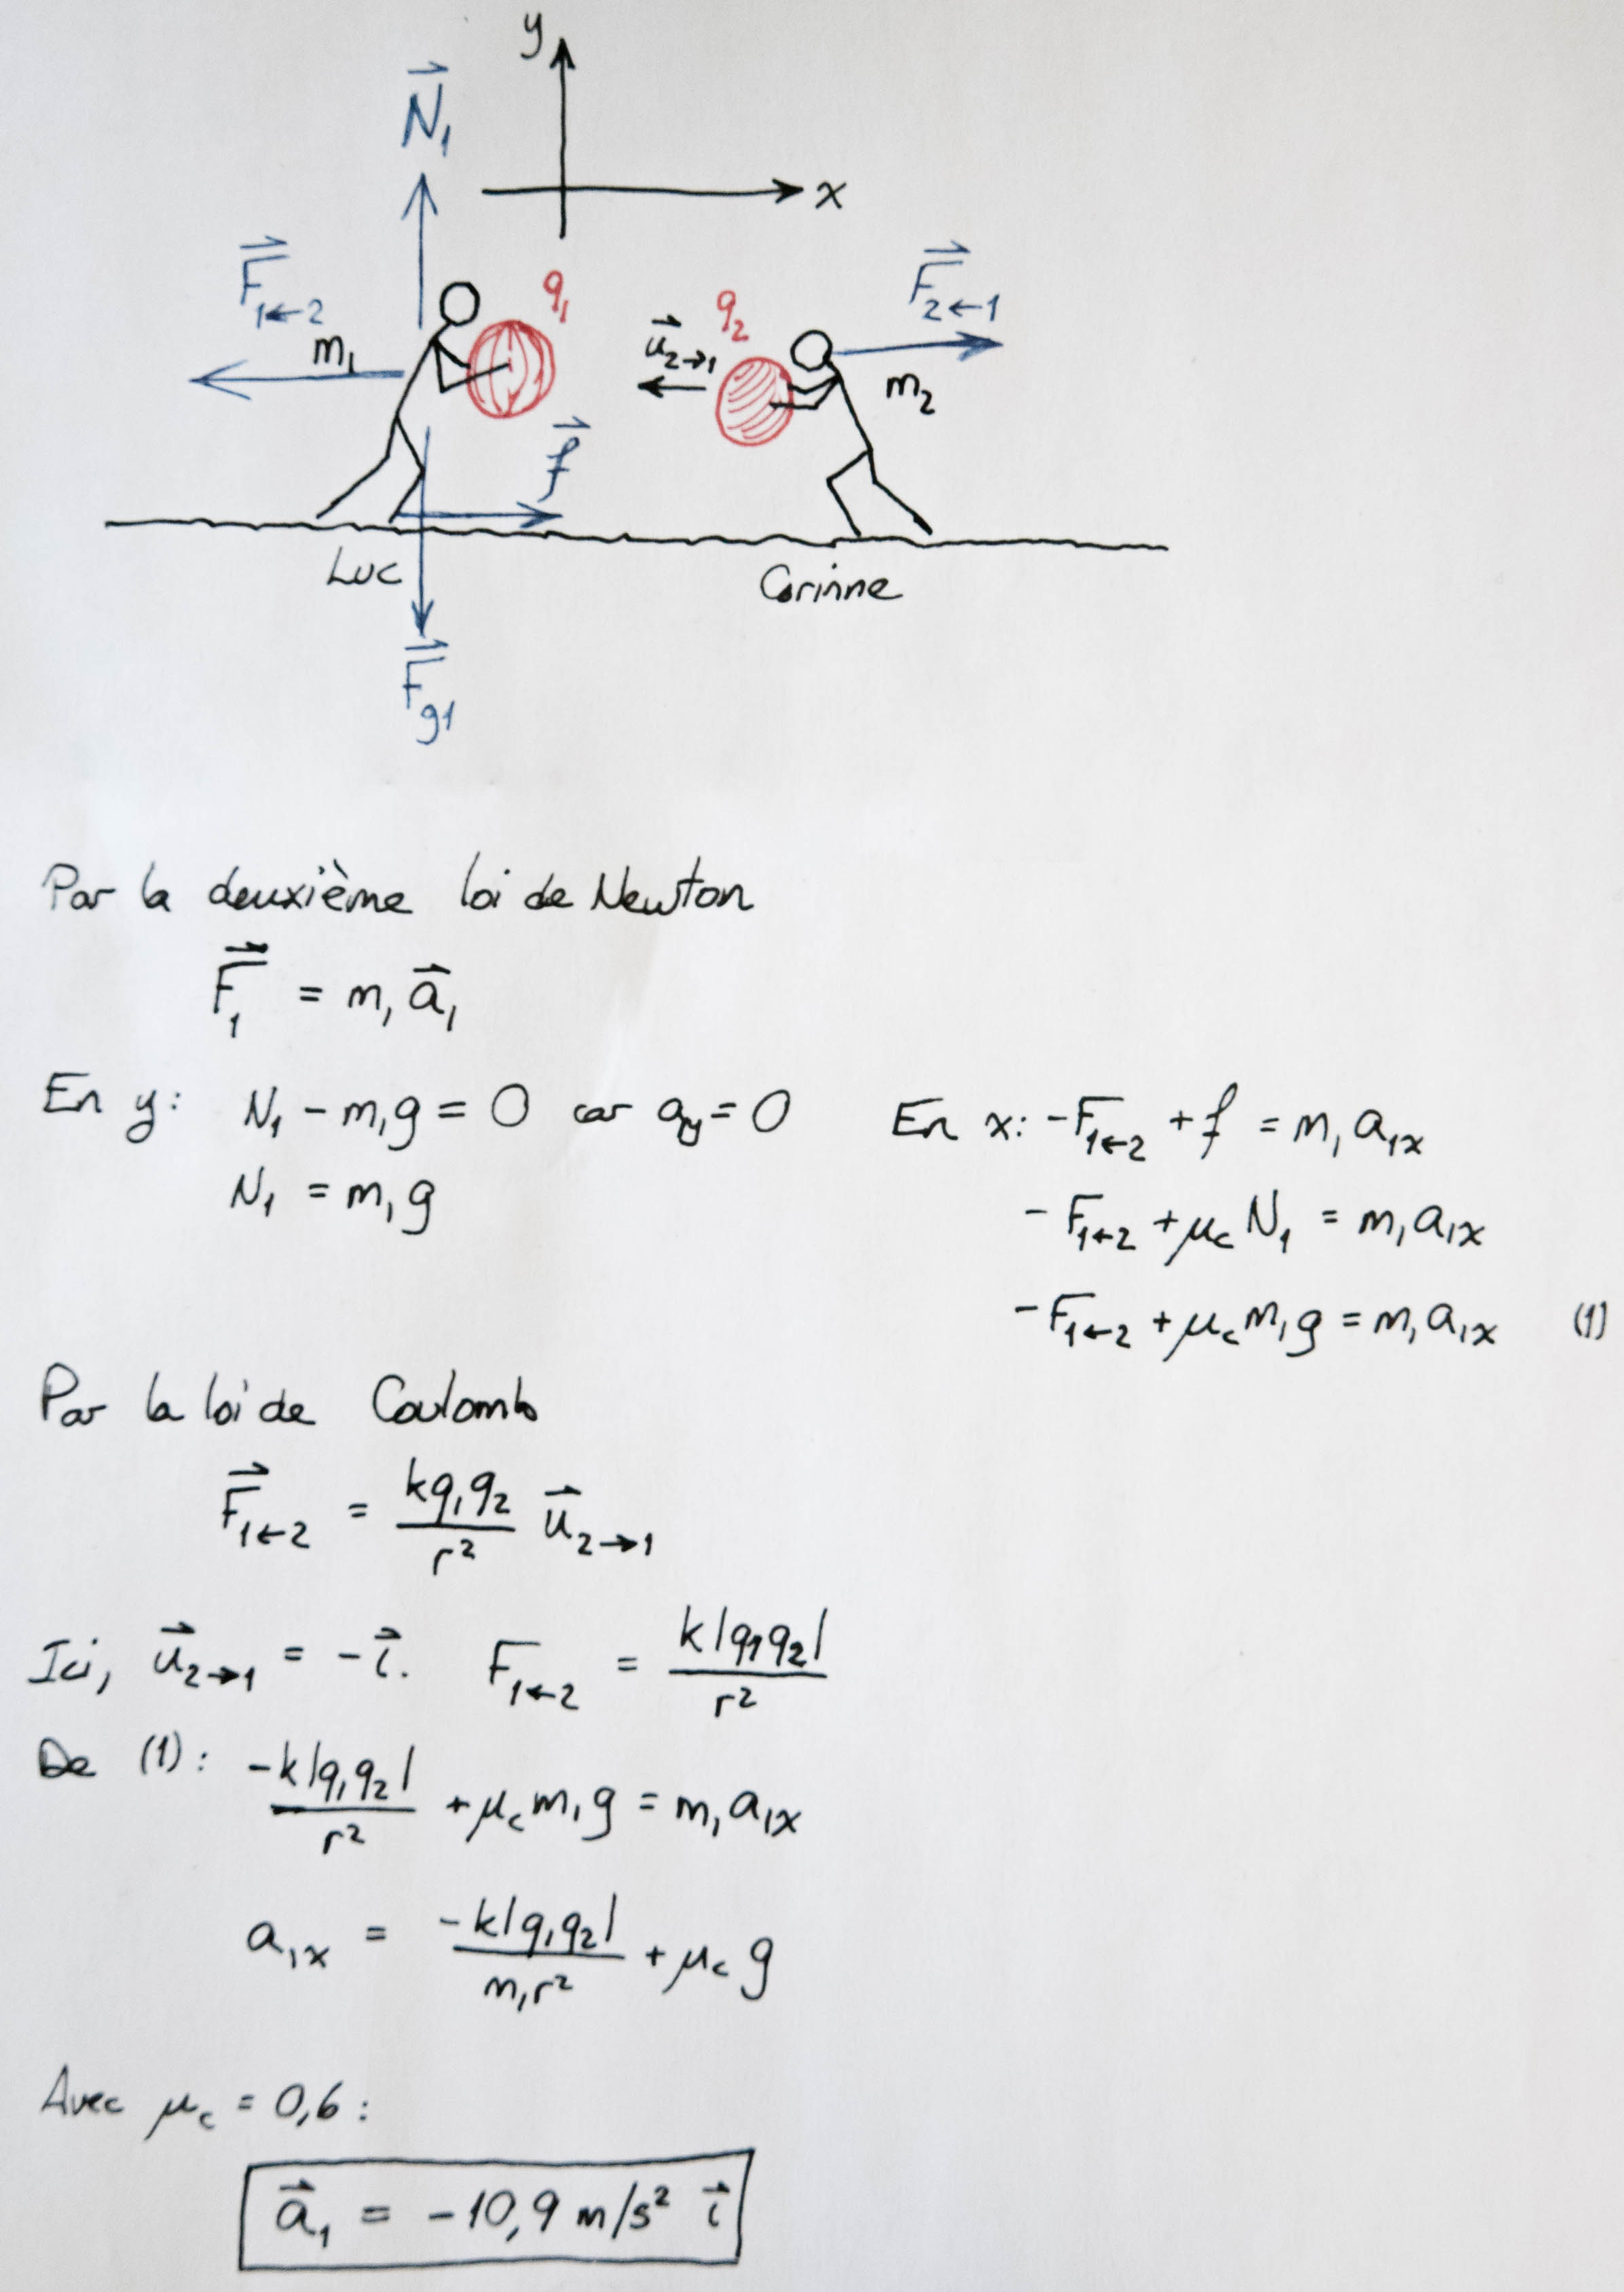
\includegraphics[scale=0.45]{figures/pousse-charge-soln.pdf}
  \end{center}

\subsection*{Loi de Coulomb 2D}

  On considère trois charges $q_1 = Q$, $q_2 = -2Q$ et $q_3 = 2Q$ placées aux
  sommets d'un triangle équilatéral de côté $d$. Une quatrième charge $q_4 =
  -Q$ est placée au centre du triangle. Déterminer la force électrostatique qui
  agit sur la charge centrale.

  La situation est illustrée ci-dessous.

  \begin{center}
  \begin{tikzpicture}
    \coordinate (center) at (2, 1.155);
    \coordinate (p1) at (2, 3.464);
    \coordinate (p2) at (0, 0);
    \coordinate (p3) at (4, 0);
    \path[fill=black!5] (0,0) -- ($(p2)!(p1)!(p3)$) -- (center) -- cycle;
    \node[circle, negative, minimum size=12mm] (q2) at (0, 0) {$-2Q$};
    \node[circle, positive, minimum size=12mm] (q1) at (2, 3.464) {$Q$};
    \node[circle, positive, minimum size=12mm] (q3) at (4, 0) {$2Q$};
    \draw (q2) -- (q3) -- (q1) -- (q2);
    \draw[dashed] (q2) -- ($(q1)!(q2)!(q3)$);
    \draw[dashed] (q1) -- ($(q2)!(q1)!(q3)$);
    \draw[dashed] (q3) -- ($(q1)!(q3)!(q2)$);
    \node[circle, draw=black!80, thick, fill=black!10] (q4) at (center) {$q_4$};
    \draw[ultra thick, ->] (q4) -- ($0.66*(q4) + 0.66*(q1)!(q2)!(q3)$);
    \draw[ultra thick, ->] (q4) -- ($0.34*(q4) + 0.66*(q3)$);
    \draw[ultra thick, ->] (q4) -- ($0.6*(q4) + 0.4*(q1)$);
  \end{tikzpicture}
  \end{center}

  Soit $\vec{F}_1$, $\vec{F}_2$ et $\vec{F}_3$ les forces électrostatiques sur
  $q_4$ dues à $q_1$, $q_2$ et $q_3$, respectivement. Puisque $q_2$ et $q_3$
  ont une charge identique en valeur absolue et sont à la même distance de
  $q_4$, les grandeurs $\vec{F}_2$ et $\vec{F}_3$ ont identiques. De plus, la
  symétrie du triangle équilatéral implique que les composantes horizontales de
  ces deux forces sont identiques et que les composantes verticales s'annulent.
  Par conséquent,
  \begin{eqnarray*}
    \vec{F}_2 + \vec{F}_3 &= 2 \cos\left( \frac{\pi}{6} \right)k
      \frac{2Q^2}{r^2}\xhat \\
    &= \frac{\sqrt{3} Q^2}{2\pi\varepsilon_0 r^2} \xhat
  \end{eqnarray*}
  où $r$ est la distance entre le centre du triangle et un de ses sommets.
  vertices, and $\xhat$ is a unit vector pointing right. À partir du triangle
  ombragé dans la figure ci-dessous, on trouve
  \begin{equation*}
    r^2 = \frac{d^2}{3}
  \end{equation*}
  ce qui implique que
  \begin{equation*}
    \vec{F}_2 + \vec{F}_3 = \frac{3\sqrt{3} Q^2}{2\pi\varepsilon_0 d^2} \xhat.
  \end{equation*}
  $\vec{F}_1$ a seulement une composante verticale
  \begin{eqnarray*}
    \vec{F}_1 &= k \frac{Q^2}{r^2} \yhat \\
    &= k \frac{3Q^2}{d^2} \yhat
  \end{eqnarray*}
  où $\yhat$ est un vecteur unitaire qui pointe vers le haut.
  La force sur $q_4$ est donc
  \begin{equation*}
    \vec{F} = \vec{F}_1 + \vec{F}_2 + \vec{F}_3 =
    \frac{3Q^2}{2\pi\varepsilon_0 d^2} \left( \sqrt{3} \xhat + \frac{1}{2}\yhat
    \right).
  \end{equation*}
